\chapter{Voltage peak transducer}
\section{Theory and related work} \label{sec:literature_voltage_peak_transducer}
The design chosen for this voltage peak transducer utilized a resistor divider network as well as a half wave precision rectifier. A resistor divider network is a series connection of two resistors and is used to decrease the magnitude of an input voltage to an acceptable level so that it can be measured. An important element in the design of this circuit is to minimise any current flow in the resistors, thus large resistor values must be chosen. A precision rectifier is an operational amplifier circuit configuration that allows a rectifier circuit to behave like an ideal diode and rectifier, an advantage of this circuit is that it allows us to rectify voltages smaller than the forward voltage of the diode.

\section{Design} \label{sec:design_voltage_peak_transducer}
%In this section, you need to capture your design, which should include the following: 
%\begin{itemize}
%  \item Design rationale, i.e. what your thinking was behind the design
%  \item Design calculations, for example to determine resistor values and capacitor values, or to check for allowed voltage and current ranges and levels. 
%  \item Circuit diagram.
%\end{itemize}
The first step in this design was to design a circuit that would step the fairly large \SI{24}{VAC} input down to a analogue voltage usable by the operational amplifier circuitry, for simplicity a simple voltage divider network was chosen. It was found that the largest differential mode input to the TLC2272 was equal to $V_{DD}=\SI{5}{V}$ and the absolute minimum input was found as $V_{EE}-\SI{0.3}{V}=\SI{-0.3}{V}$ \ref{yourmom}. It was also found that each TLC2272 chip required roughly \SI{2.4}{\milli A} at room temperature given a supply voltage $V_{DD}=\SI{5}{V}$. Referring to Figure \ref{fig:system_diagram} we can see that this design required two of these chips, and thus it was decided that for the voltage transducer a single supply would be used as to not exceed the limitations of the negative voltage supply rail specified in the first report. 
Given this information a 1N4007 diode was placed in series with the voltage divider as to not exceed the maximum negative differential mode input of \SI{-0.3}{V}. Choosing an absolute maximum input voltage of \SI{24}{VAC}, and compensating for the forward voltage of the diode, the input to the resistor divider network was found to be $V_{in}=\SI{23.3}{VAC}$. To keep power losses to a minimum $R_{2}=\SI{10}{\kilo \Omega}$ was chosen, The value of $R_{1}$ can be found by using Equation \ref{eq:voltagedivider}. After rearranging the terms and substituting for the values, it was found that $R_{1}=\SI{56.6}{\kilo \Omega}$, which is very close to the chosen standard resistor value of $\SI{56}{\kilo \Omega}$.\newline
\begin{align}
   V_{DD}=\frac{R_2}{R_1+R_2}V_{in}
   \label{eq:voltagedivider}
\end{align}
The peak detection circuit chosen for this design was a simple precision rectifier as can be seen in Figure \ref{fig:voltagepeakdetector.pdf}. To minimise any power losses in the operational amplifier, a resistor $R_3=\SI{10}{\kilo \Omega}$ was placed at its positive input pin to prevent an excess amount of current from flowing into the operational amplifier. It is worth noting that if any negative voltages are applied at the input of the precision rectifier the operational amplifier runs open loop since the diode is reverse biased, this causes the operational amplifier to saturate. It takes time for the operational amplifier to move out of saturation, and this greatly decreases the frequency response of the circuit, thus further motivating the choice of supplying the operational amplifier with a single supply configuration. \vspace{4mm} \newline
The Arduino's pins work with a voltage level of $\SI{5}{V}$ and the resistor divider network outputs a voltage of up to $\SI{5}{V}$ we require the operational amplifier to have a gain of 1, thus a feedback resistor $R_4$ with a resistance equal to that of $R_3$ had to be placed between the negative input pin and the anode of the diode.
The final part of the peak detection circuit requires a capacitor and resistor with an adequate RC constant as to maintain the desired peak voltage to be measured by the Arduino. A chosen ripple voltage of no more than $\SI{5}{\milli V}$ was chosen for this design and the required capacitor could then be found by applying Equation \ref{eq:ripplevoltage}. With a maximum input voltage $V_{m}=\SI{5}{V}$, a frequency of \SI{50}{Hz}, the internal resistance of the Arduino's pins $R=\SI{1}{M\Omega}$ we can see that the desired capacitor value needs to be equals to $C=\SI{20}{\micro F}$.\newline
\begin{align}
  V_{r} = \frac{V_{m}}{fRC} 
   \label{eq:ripplevoltage}
\end{align}
Given the specification of a maximum input voltage of $\SI{24}{VAC}$ corresponding to a voltage of $\SI{5}{VAC}$ and the Arduino having a range of $4095$ bits, it can be calculated that the resolution of the ADC would be $\SI{8.1175}{\milli V}$ per bit, taking the forward voltage of the rectifier diode into consideration. To ensure that the transducer met the design requirement of responding to a $\SI{1}{V}$ change, which corresponds to an output voltage change of $\SI{151.15}{\milli \volt}$, within 1 second, Equation \ref{eq:capacitordischarge} had to be used. Here $V_{s}=\SI{3.4284}{\volt}$, which corresponds to an input of \SI{16}{VAC}, and $V_{c}=\SI{3.2769}{\milli \volt}$, which corresponds to a \SI{1}{V} decrease in input peak voltage. Using Equation \ref{eq:capacitordischarge} an appropriate smoothing capacitor could be chosen, as the equivalent input resistance of the Arduino was equal to $R=\SI{1}{M \Omega}$ and with the voltage changes measured before the capacitor was found to be $C=\SI{22.12}{\micro F}$. To minimize noise on the output of this transducer two low ESR rated \SI{10}{\micro F} capacitors were placed in parallel to make an equivalent capacitance of \SI{20}{\micro F}. Decoupling capacitors were also placed at the positive voltage supply input to the TLC2272 to minimize any effects of noise from the power supply on the output of the transducer.
\begin{align}
  V_{c} = V_{s}e^{\frac{-t}{RC}} \\
  C = \frac{t}{(\ln(\frac{V_{s}}{V_{c}}))R} \nonumber
   \label{eq:capacitordischarge}
\end{align}

\begin{figure}[h!]
    \centering
    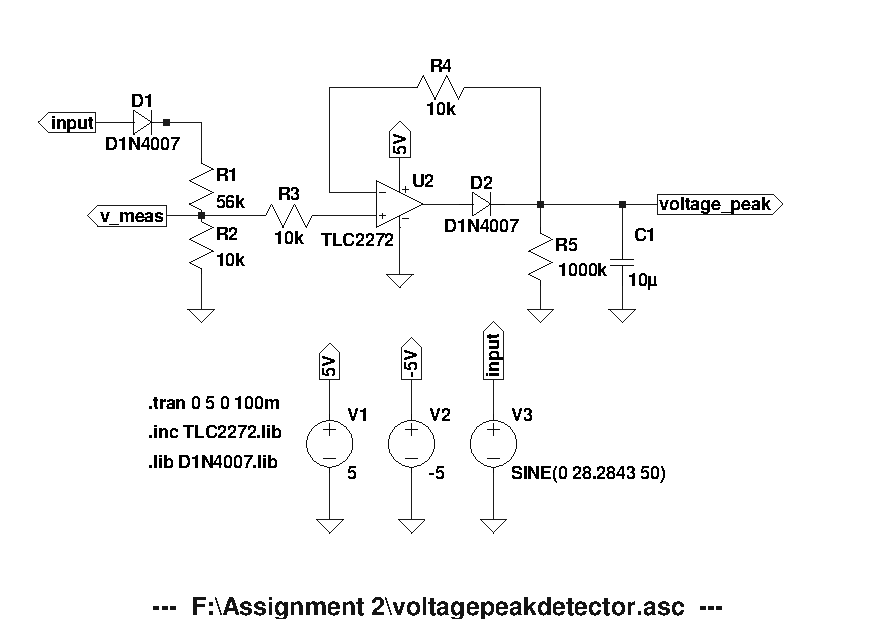
\includegraphics[width = 0.65\linewidth]{Figures/voltagepeakdetector.pdf}
        \caption{Voltage Peak Transducer Diagram}
    \label{fig:voltagepeakdetector.pdf}
\end{figure}


\section{Simulation} \label{sec:simulation_voltage_peak_transducer}
%In this section, you want to demonstrate, by means of simulation results, using the designed circuit, what your circuit is expected to behave. An example is the figure shown in Figure \ref{fig:simulation_results_box} or Subfigure \ref{subfig:AC}. Be absolutely sure that the text and information in your report are readable. 
Firstly the designed voltage transducer was simulated given a nominal input voltage of $\SI{16}{VAC}$ and the plot of this output can be seen in Figure \ref{subfig:16VACinputripple}. From the graph it can be deduced that at steady state a ripple voltage of $V_{c}=\SI{13.28}{\milli \volt}$ can be expected, this is slightly higher than the ripple voltage designed for in the previous section, however for the purpose of this design this was deemed acceptable. The next result that was simulated was the voltage transducers response to a $\SI{1}{\volt}$ change in a $\SI{16}{VAC}$ input, this was done by using a piece wise linear voltage source to decrease the input voltage by $\SI{1}{\volt}$, this output can be seen in Figure \ref{subfig:16VACinputchange}. From this graph we can see that the voltage transducer responded to the change in input in exactly 1 second, which confirms that it responded as was expected.

\begin{figure}[h!]
 \centering
     \begin{subfigure}[]{0.45\textwidth}
        \centering
         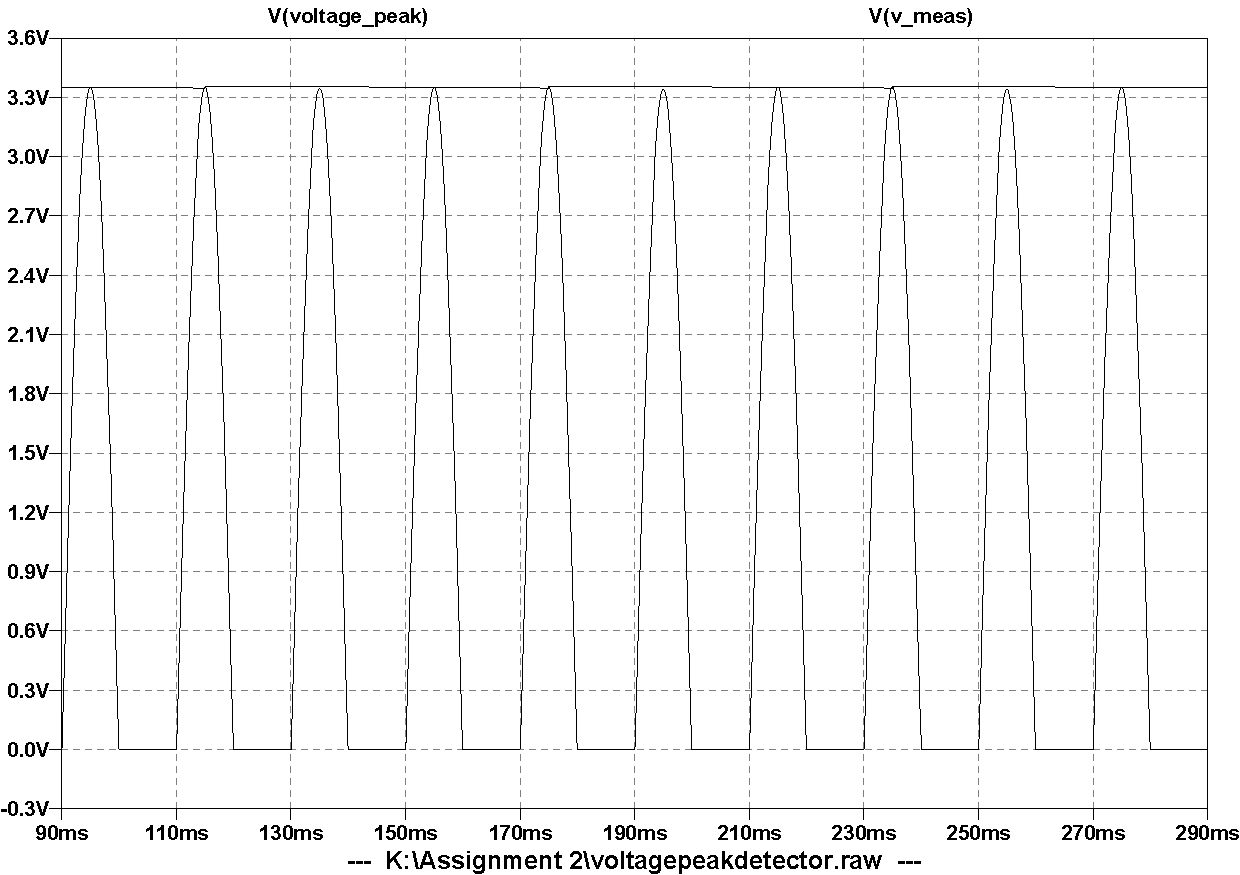
\includegraphics[width=1\linewidth]{./Figures/voltagepeakdetectoroutputsim.pdf}
		    \caption{Peak detection of scaled down \SI{16}{\volt AC} input.} \label{subfig:16VACinputripple}
     \end{subfigure}
      \begin{subfigure}[]{0.45\textwidth}
              \centering
  		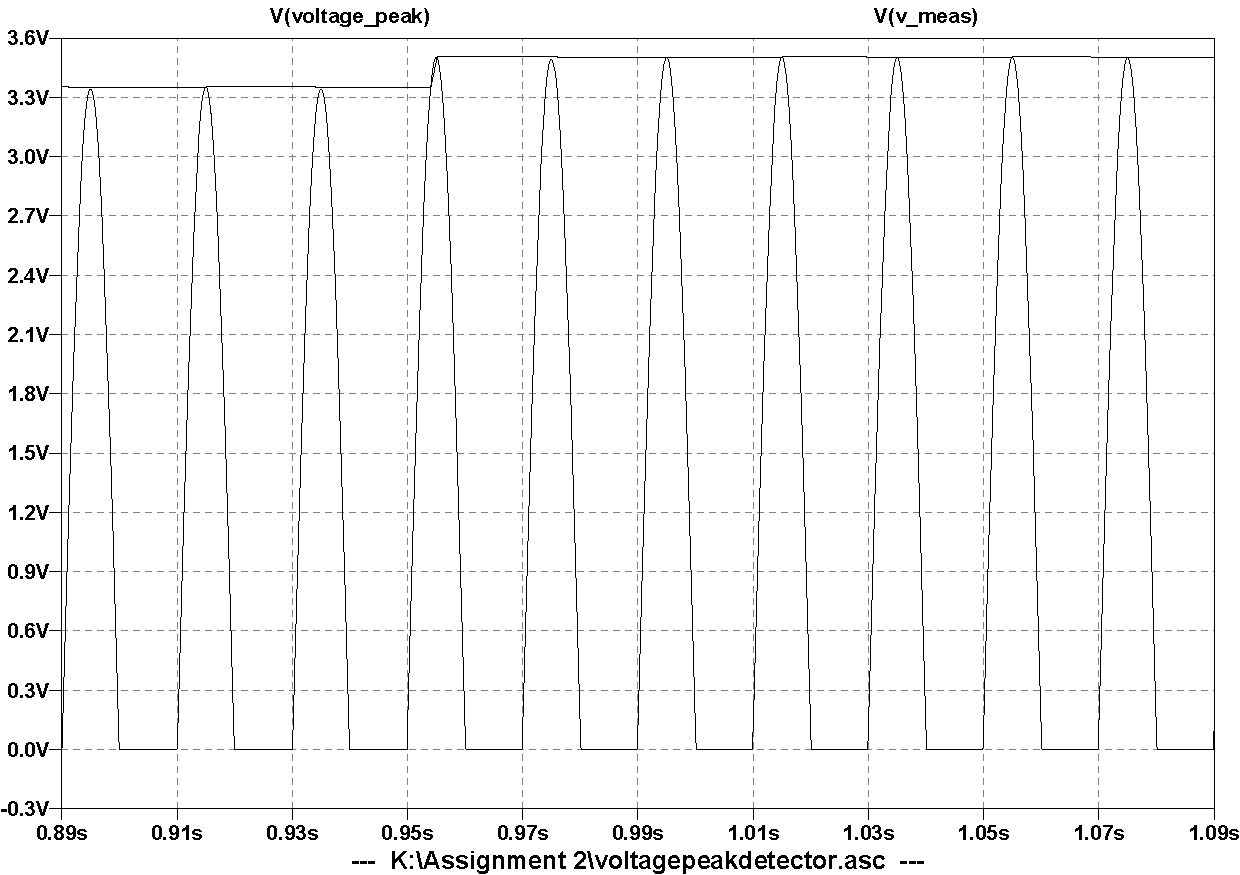
\includegraphics[width=1\linewidth]{./Figures/voltagepeakdetectoroutputchange.pdf}
		    \caption{Response given \SI{1}{\volt} change in \SI{16}{\volt AC} input.} \label{subfig:16VACinputchange}
     \end{subfigure}
   \caption[Simulated results for the voltage transducer]{Output voltage ripple and response for the voltage transducer. (a) depicts output voltage ripple, (b) depicts response to change in input. }
    \label{fig:simulation_results_box}
 \end{figure}

\section{Measurements} \label{sec:measurement_voltage_peak_transducer}

%In this section, you must present your measured results. You can use screengrabs or photos of the oscilloscope, or download the CSVs and plot them as PDFs using Matlab, Excel or similar. 
Unit tests were completed using a signal generator applied at the input of the voltage peak transducer to simulate various input voltages, these results can be seen in Table \ref{tab:voltagetransducerunittests}. All unit test measurements were measured accurately and the simulated input was deduced using Equation 2.4 with a maximum difference of only $\SI{83.12}{\milli \volt}$. The transducer was then tested using the transformer as input under various load conditions and these results can be seen in Table \ref{tab:voltagetransducerrealtests}. Under all load conditions the deduced input differed from the actual input by no more than $\SI{118}{\milli \volt}$, confirming that the design met all requirements. The output of the voltage peak transducer given an input from the transformer, with a load of $\SI{1}{\kilo \Omega}$ can be seen in Figure \ref{subfig:voltagetransducermidrange}, with the quality of this signal shown in Figure \ref{subfig:16VACinputchange}. From this it was found that the transducer can accurately detect the peak of an input voltage with a maximum output noise below $\SI{10}{\milli \volt}$.
\begin{align}
  V_{meas} = (V_{in}-V_{\gamma}) * \frac{R_1}{R_1+R_2} \\
  V_{meas} = (V_{in}-0.7) * 0.14374 \nonumber
   \label{eq:pleaseworkthistime}
\end{align}

\newcolumntype{C}[1]{>{\centering\arraybackslash}m{#1}}
\begin{table} [h!]
        \centering
        \footnotesize
        \caption{Voltage transducer intermediate unit test results.}
             \begin{tabular}{C{2cm} C{2cm} C{2cm} C{2cm} C{2cm} C{2cm}}
           Emulated level & Signal generator & Signal generator & Analogue output & Deduced input & Difference \\
           ($V_{peak}$)   & ($V_{peak}$)   & ($V_{peak}$)   & ($VDC$)         & ($V_{peak}$)  & ($mV_{peak}$) \\
           \hline
            16      & 2.194 & 2.196 & 2.208 & 16.081 & 83.12 \\
            21      & 2.192 & 2.915 & 2.916 & 21.009 & 8.67\\
            21.15   & 2.931 & 2.936  & 2.940 & 21.174 & 23.55 \\
            21.30   & 2.954 & 2.958 & 2.960 & 21.318 & 17.98 \\
            26      & 3.629 & 3.634 & 3.626 & 25.946 & 53.96\\
          \hline
        \end{tabular}
     \label{tab:voltagetransducerunittests}
\end{table}

\begin{table}
        \centering
        \footnotesize
        \caption{Voltage transducer integrated test results.}
         \begin{tabular}{C{1.9cm} C{1.2cm} C{1.2cm} | C{2.5cm} C{2.6cm} C{2.5cm} C{1.8cm}}
           Measurement & Load R & Load C  & Measured input & Analogue output & Deduced input & Difference\\
            & ($\Omega$) & ($\mu F$) & ($V_{peak}$) & ($VDC$) & ($V_{peak}$) & ($mV_{peak}$) \\
        \hline
            No load      & open & none & 30.38 & 4.270 & 30.406  & 26 \\
            Full load    & 100  & none & 29.12 & 4.140 & 29.224  & 104 \\
            Mid range    & 1k   & none & 30.08 & 4.240 & 30.198  & 118\\
          \hline
        \end{tabular}
     \label{tab:voltagetransducerrealtests}
\end{table}

\begin{figure}[h!]
 \centering
     \begin{subfigure}[]{0.45\textwidth}
        \centering
         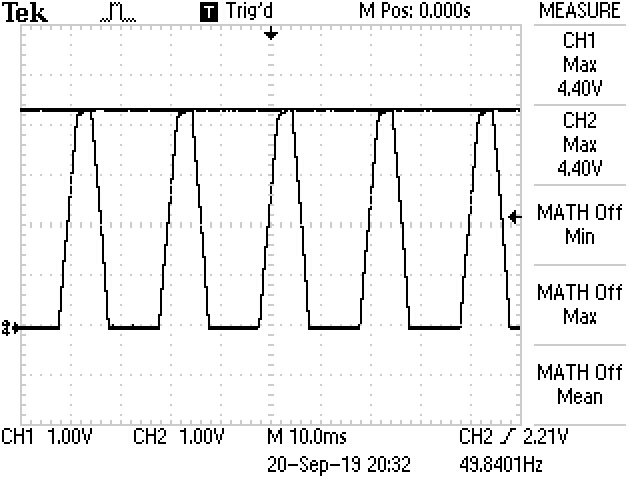
\includegraphics[width=1\linewidth]{./Figures/voltagetransducermidrange.JPG}
		    \caption{Mid range measurement result} \label{subfig:voltagetransducermidrange}
     \end{subfigure}
      \begin{subfigure}[]{0.45\textwidth}
              \centering
  		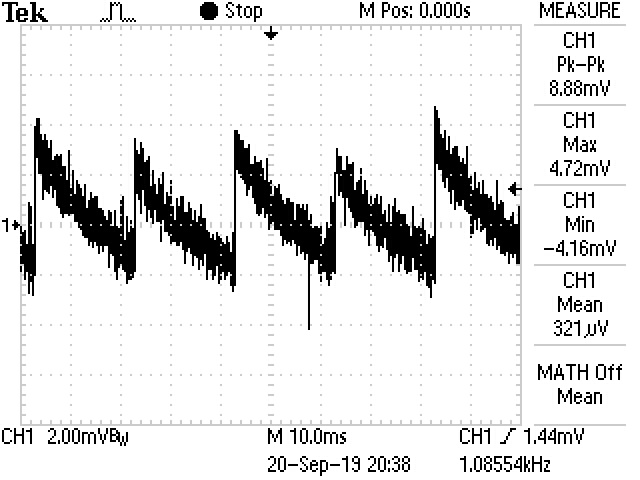
\includegraphics[width=1\linewidth]{./Figures/voltagetransducernoise.JPG}
		    \caption{Noise response} \label{subfig:16VACinputchange}
     \end{subfigure}
   \caption[Measured results for the voltage transducer]{Output voltage ripple and response for the voltage transducer. (a) depicts mid range output, (b) depicts noise response. }
    \label{fig:simulation_results_box}
 \end{figure}